\documentclass[preprint,5p,times]{elsarticle}
\usepackage {amsmath}
\usepackage {epsfig}
\usepackage {graphicx}
\usepackage{booktabs}

%%\usepackage[spanish]{babel}   %
%%\selectlanguage{spanish}      %  Españól
%%\usepackage[utf8]{inputenc}   %
\usepackage {framed,color}
\makeatletter
\def\verbatim{\small\@verbatim \frenchspacing\@vobeyspaces \@xverbatim}
%\def\verbatim{\scriptsize\@verbatim \frenchspacing\@vobeyspaces \@xverbatim}
\makeatother

%\usepackage{mathpazo}
\journal{Soil Dynamics and Earthquake Engineering}

\begin{document}

\begin{frontmatter}
\title{The tunnel-shaft earthquake response in layered soils using a hybrid Discrete Wavenumber and Indirect Boundary Element Method}
\author{the team}
%\author[unam]{Marcial Contreras-Zazueta}
\ead{marcialcz@iingen.unam.mx}
%\address[unam]{Universidad Nacional Autónoma de México, Av. Universidad 1900, Coyoacán Ciudad de México, México}

\begin{abstract}
Displacement demands in the tunnel and shafts of a deep underground drainage system in a soft layered valley are studied with a hybrid indirect boundary element and discrete wavenumber method. The use of a Green's function for the layered soil allows the boundary element problem to be solved with far less collocation points. Our optimized algorithm is attractive for the study of several engineering problems too costly or too cumbersome with current techniques. 
\end{abstract}
\begin{keyword}
tunnel-shaft \sep IBEM \sep DWN\sep layered soil \sep displacement demands
\end{keyword}
\end{frontmatter}
\section{Introduction}

\section{Reducing the boundary element problem}
In a multi-domain space an elastic wave will propagate through different media, most commonly parallel strata and inclusions. Given a wavelength of interest we can distinct the observable inclusions $m^{(d)}$ from $m^{(l)}$ a stack of horizontal homogeneous layers over a half-space. For this configuration it is convenient to lump the strata response in a single Green's function, then solve only for the diffraction of $m^{(d)}$ in an equivalent homogeneous full-space. The total displacement field would be,
\begin{equation}
u = u^{(0)} + u^{(l)} + u^{(d)},
\end{equation}
where $u^{(0)}$ is the incident field, $u^{(l)}$ is the field diffracted by the layered half-space which we discuss in section~\ref{sec:layeredhalfspaceGreenfunc}, and $u^{(d)}$ is the field diffracted by the inclusions $m^{(d)}$. The indirect formulation of the boundary element method (IBEM) \cite{Sanchez-sesma1995} is used to readily obtain the diffracted displacement and traction fields with the following corresponding expressions,
\begin{equation}
\begin{aligned}
u_i^{(d)}(\boldsymbol{x}) = \int_{\partial \Gamma} \phi^{(d)}_j(\boldsymbol{\xi}) G_{ij}^{(l)} (\boldsymbol{x},\boldsymbol{\xi}) d S_{\xi},\\
t_i^{(d)}(\boldsymbol{x}) = \int_{\partial \Gamma} \phi^{(d)}_j(\boldsymbol{\xi}) T_{ij}^{(l)} (\boldsymbol{x},\boldsymbol{\xi}) d S_{\xi},
\end{aligned}
\end{equation}
where $\partial \Gamma$ are the joint continuous surfaces of $m^{(d)}$, $G_{ij}^{(l)}(\boldsymbol{x},\boldsymbol{\xi})$ and $T_{ij}^{(l)}(\boldsymbol{x},\boldsymbol{\xi})$ are the layered half-space Green's functions for displacement and traction for a known normal respectively, i.e., the response in the direction $i$ at point $\boldsymbol{x}$ in layer $l(x)$ due to the application of a unit force in the direction $j$ at point $\boldsymbol{\xi}$ in layer $l(\xi)$, and $\phi_j(\boldsymbol{\xi})$ force density in the $j$ direction. 

The refracted field inside $m^{(d)}$ is obtained from an analogous boundary integral again on $\partial \Gamma$,
\begin{equation}
\begin{aligned}
u_i^{(r)}(\boldsymbol{x}) = \int_{\partial \Gamma} \phi^{(r)}_j(\boldsymbol{\xi}) G_{ij}^{(0)} (\boldsymbol{x},\boldsymbol{\xi}) d S_{\xi},\\
t_i^{(r)}(\boldsymbol{x}) = \int_{\partial \Gamma} \phi^{(r)}_j(\boldsymbol{\xi}) T_{ij}^{(0)} (\boldsymbol{x},\boldsymbol{\xi}) d S_{\xi},
\end{aligned}
\end{equation}
where $G_{ij}^{(0)}(\boldsymbol{x},\boldsymbol{\xi})$ and $T_{ij}^{(0)}(\boldsymbol{x},\boldsymbol{\xi})$ are the displacement and traction Green's functions for the inclusion materials. We consider the $m^{(d)}$ domain to be homogeneous but it may as well be of the layered kind.

The unknown force densities $\phi^{(d)}(\boldsymbol{\xi})$ and $\phi^{(r)}(\boldsymbol{\xi})$ are solved on discretized $\partial\Gamma$ from the continuity and free-field boundary conditions,
\begin{equation}
\begin{aligned}
u^{(0)} + u^{(l)} + u^{(d)} =  u^{(r)} && \mathrm{at} && \partial_2 \Gamma, \\
t^{(0)} + t^{(l)} + t^{(d)} =  t^{(r)} && \mathrm{at} && \partial_2 \Gamma, \\
t^{(r)} = 0 && \mathrm{at} && \partial_1 \Gamma,
\end{aligned}
\end{equation}
with $\partial_1 \Gamma$ the free surface of $m^{(d)}$ and $\partial_2 \Gamma$ the common boundary with $m^{(l)}$. The null tractions condition at the surface is already satisfied by the layered half-space Green's functions and we consider only inclusions that do not share a boundary with another inclusion. An optimized algorithm for the determination of boundary conditions of complex two-dimensional multi-domain geometries was recently published by [art the Mathieu].


\section{Layered half-space Green's function}
\label{sec:layeredhalfspaceGreenfunc}
Consider the stack of $N$ horizontal, elastic, homogeneous, isotropic layers over a half-space. On a given $l$-th layer defined at $z_l \le z < z_{l+1}$, the displacement and traction fields at point $\boldsymbol{x}$, due to a unit force at point $\boldsymbol{\xi}$ are,
\begin{equation}
\begin{aligned}
u^{(0)} \delta(l,l(\boldsymbol{\xi})) + u^{(l)}, \\
t^{(0)} \delta(l,l(\boldsymbol{\xi})) + t^{(l)},
\end{aligned}
\label{us}
\end{equation}
where $\delta$ is Kronecker's delta and tractions are taken on a surface with known normal vector $\boldsymbol{n}$.

% campo incidente
In a cylindrical coordinate system the full-space displacement function admits an integral representation over the radial wave number $k$ with the following form for the vertical load case,
\begin{equation}
	 \left[\begin{matrix} -i u_z^{(0)} \\
	 k u_r^{(0)} \end{matrix} \right] = \int_{0}^{\infty}\frac{k}{4 \pi \rho \omega^2} \boldsymbol{H}_v(r) \boldsymbol{A}_v(z) dk,
	 \label{Gij0_k_hor}
\end{equation}
and for the horizontal load case,
\begin{equation}
\begin{aligned}
\left[\begin{matrix} -i u_z^{(0)} \\
k u_r^{(0)} \end{matrix} \right] = \int_{0}^{\infty}\frac{k}{4 \pi \rho \omega^2} \left(\boldsymbol{H}_h(r) \boldsymbol{A}_h(z) + \boldsymbol{H}_s(r) \boldsymbol{A}_s(z)\right) dk, \\
k u_\theta^{(0)} = \int_{0}^{\infty}\frac{\mu k}{4 \pi \rho \omega^2} \left(\boldsymbol{H}_h^\theta(r) \boldsymbol{U} \boldsymbol{A}_h(z) + \boldsymbol{H}_s^\theta(r) \boldsymbol{A}_s^\theta(z)\right) dk,
\end{aligned}
\end{equation}
where $\rho$ = mass density, $\omega$ = circular frequency, $i^2=-1$,
\begin{equation}
\begin{aligned}
  \boldsymbol{H}_v(r) = \left[\begin{matrix}
    J_0 & 0 \\ 0 & k\ J_1 
    \end{matrix} \right], \\
  \boldsymbol{A_v}(z) = \left[\begin{matrix}
    -\gamma & -\left(k^2/\nu\right) \\ -sgn(z)\ k & sgn(z)\ k 
    \end{matrix} \right] \left[\begin{matrix}
    e^{-i \gamma |z|} \\ e^{-i \nu |z|}
    \end{matrix} \right],\\
  \boldsymbol{H}_h(r) = \left[\begin{matrix}
    k\ J_1 \cos \theta & 0 \\ 0 & - k (J_0 - J_1/kr)\cos \theta 
    \end{matrix} \right], \\
  \boldsymbol{A_h}(z) =  \left[\begin{matrix}
    i\ sgn(z) & - i\ sgn(z) \\ i k^2/\gamma &  i \nu
    \end{matrix} \right] \left[\begin{matrix}
    e^{-i \gamma |z|} \\ e^{-i \nu |z|}
    \end{matrix} \right], \\
  \boldsymbol{H}_s(r) = \left[\begin{matrix}
    0 \\ k J_1 \cos \theta / kr
    \end{matrix} \right], \\
  \boldsymbol{A_s}(z) =  \begin{matrix}
	-i \left(\omega^2 /\nu \beta^2 \right) e^{-i \nu |z|}
	\end{matrix}, \\
  \boldsymbol{H}_h^\theta(r) =k \sin \theta J_1/kr, \\
  \boldsymbol{U} = \left[\begin{matrix} 0 & 1 \end{matrix}\right], \\
   \boldsymbol{H}_s^\theta(r) =  k (J_0 - J_1/kr)\sin \theta, \\
   \boldsymbol{A_s}^\theta(z) = -\boldsymbol{A_s}(z),
\end{aligned}
\end{equation}
where $\gamma^2 = \omega^2 / \alpha^2 - k^2$, $ Im(\gamma) \le 0$, $\nu^2 = \omega^2 / \beta^2 - k^2$, $ Im(\nu) \le 0$, $\alpha$ = P-wave velocity, $\beta$ = S-wave velocity, $r^2 = (x_1 - \xi_1)^2 + (x_2 - \xi_2)^2$,$\tan \theta = (x_2 - \xi_2) / (x_1 - \xi_1)$, $z = x_3 - \xi_3$, $sgn$ is the sign function and $J_n = J_n(kr)$ is the Bessel function of the first kind and order $n$.

The corresponding Green's tractions on a horizontal surface for a vertical force,
\begin{equation}
\left[\begin{matrix} k \sigma_{zz}^{(0)} \\
ik \sigma_{zr}^{(0)} \end{matrix} \right] = \int_{0}^{+ \infty} \frac{\mu k}{4 \pi \rho \omega^2} \boldsymbol{Q}_v(r) \boldsymbol{B}_v(z) dk,
\label{Tij0_k_ver}
\end{equation}
and for a horizontal force,
\begin{equation}
\begin{aligned}
\left[\begin{matrix} k \sigma_{zz}^{(0)} \\
ik \sigma_{zr}^{(0)} \end{matrix} \right] = \int_{0}^{\infty}\frac{\mu k}{4 \pi \rho \omega^2} \left(\boldsymbol{H}_h(r) \boldsymbol{B}_h(z) + \boldsymbol{H}_s(r) \boldsymbol{B}_s(z)\right) dk, \\
ik \sigma_{z \theta}^{(0)} = \int_{0}^{\infty}\frac{\mu k}{4 \pi \rho \omega^2} \left(\boldsymbol{H}_h^\theta(r) \boldsymbol{U} \boldsymbol{B}_h(z) + \boldsymbol{H}_s^\theta(r) \boldsymbol{B}_s^\theta(z)\right) dk,
\end{aligned}
\label{Tij0_k_hor}
\end{equation}
where $\mu = \rho \beta^2$, $\eta = k^2-\nu^2$,
\begin{equation}
\begin{aligned}
\boldsymbol{Q}_v(r) = \left[\begin{matrix}
k J_0 & 0 \\ 0 & k J_1
\end{matrix}\right] \\
\boldsymbol{B_v}(z) = \left[\begin{matrix}
sgn(z) \eta & -sgn(z)2k^2 \\ -2\gamma k & -k \eta / \nu 
\end{matrix} \right] \left[\begin{matrix}
e^{-i \gamma |z|} \\ e^{-i \nu |z|}
\end{matrix} \right],\\
\boldsymbol{B_h}(z) = \left[\begin{matrix}
-ik\eta /\gamma & -2ik\nu \\ i sgn(z)2k^2 & -i sgn(z)\eta 
\end{matrix} \right] \left[\begin{matrix}
e^{-i \gamma |z|} \\ e^{-i \nu |z|}
\end{matrix} \right],\\
\boldsymbol{B}_s(z) = -i sgn(z) (\omega / \beta)^2 e^{-i \nu |z|},\\
\boldsymbol{B}_s^\theta(z) = - \boldsymbol{B}_s(z)
\end{aligned}
\end{equation}

%luego campo difractado
The displacement field diffracted by the layered half-space can be expressed in terms of potentials for dilatational and shear waves \cite{Knopoff1964} \cite{Aki1980} allowing an integral representation on the radial wavenumber. From \cite{Sanchez-sesma2011a} the diffracted field of displacements at layer $l$ have the following compact form for the vertical load case is,
\begin{equation}
		\left[\begin{matrix} -i u_z^{(l)} \\
		k u_r^{(l)} \end{matrix} \right] = \int_{0}^{+ \infty} \boldsymbol{H}_v(r)\boldsymbol{F}^{(l)}(z) \boldsymbol{X} dk,\\
		\label{eqUdifver}
\end{equation}
and for the horizontal load case,
\begin{equation}
\begin{aligned}
\left[\begin{matrix} -i u_z^{(l)} \\
k u_r^{(l)} \end{matrix} \right] = \int_{0}^{+ \infty} \left(\boldsymbol{H}_h(r) \boldsymbol{F}^{(l)}(z) \boldsymbol{X} + \boldsymbol{H}_s(r) \boldsymbol{C}^{(l)}(z) \boldsymbol{Y}\right) dk, \\
k u_\theta^{(l)} = \int_{0}^{+ \infty} \left(\boldsymbol{H}_h^\theta(r) \boldsymbol{U} \boldsymbol{F}^{(l)}(z) \boldsymbol{X} - \boldsymbol{H}_s^\theta(r) \boldsymbol{C}^{(l)}(z) \boldsymbol{Y}\right) dk,
\end{aligned}
\label{eqUdifhor}
\end{equation}
where,
\begin{equation}
	\begin{aligned}
\boldsymbol{F}^{(l)}(z) = \left[\begin{matrix}
	-\gamma & -k & +\gamma & -k \\
	-k  & \nu & -k  & -\nu 
	\end{matrix} \right] \boldsymbol{D},\\
\boldsymbol{D} = diag\left(\begin{matrix}
	\exp(-i\gamma (z-z_l)) \\
	\exp(-i \nu (z-z_l)) \\
	\exp(+i\gamma(z-z_{l+1})) \\
	\exp(+i \nu (z-z_{l+1})) 
	\end{matrix} \right), \\
\boldsymbol{C}^{(l)}(z) = \left[\begin{matrix}
k & k
\end{matrix}\right] \left[\begin{matrix}
e^{-i \nu (z-z_l)} \\ e^{i \nu (z-z_{l+1})}
\end{matrix} \right],\\
	\end{aligned}
\end{equation}
where $diag(a_1,...,a_n)$ is a diagonal matrix whose entries starting in the upper left corner are $a_1,...,a_n$, and the coefficients vectors,
\begin{equation}
\begin{aligned}
	\boldsymbol{X} = \left[\grave{P},ik\grave{V},\acute{P},ik\acute{V} \right]^T,\\
	\boldsymbol{Y} = \left[\grave{T},\acute{T}\right]^T,
	\end{aligned}
	\label{eqIncognitas}
\end{equation} 
where $P,V,T$ correspond to P, SV and SH plane wave amplitudes respectively and the acute and grave accents indicate up going or down going propagation respectively. At layer $(l)$, up going waves are emitted from the deeper interface $l+1$ while down going waves are emitted form the shallower interface $l$. Sommerfeld's radiation condition implies no diffracted up going waves are expected in a half-space. 

The corresponding Green's tractions on a horizontal surface for a vertical force,
\begin{equation}
\left[\begin{matrix} k \sigma_{zz}^{(l)} \\
ik \sigma_{zr}^{(l)} \end{matrix} \right] = \int_{0}^{+ \infty} \mu \boldsymbol{Q}_v(r) \boldsymbol{S}^{(l)}(z) \boldsymbol{X} dk,
\label{eqTdifver}
\end{equation}
and for a horizontal force,
\begin{equation}
\begin{aligned}
\left[\begin{matrix} k \sigma_{zz}^{(l)} \\
ik \sigma_{zr}^{(l)} \end{matrix} \right] = \int_{0}^{\infty} \mu \left(\boldsymbol{H}_h(r) \boldsymbol{S}^{(l)}(z)\boldsymbol{X} + \boldsymbol{H}_s(r) \boldsymbol{E}^{(l)}(z) \boldsymbol{Y}\right) dk, \\
ik \sigma_{z \theta}^{(l)} = \int_{0}^{\infty} \mu \left(\boldsymbol{H}_h^\theta(r) \boldsymbol{U}\boldsymbol{S}^{(l)}(z)\boldsymbol{X} - \boldsymbol{H}_s^\theta(r) \boldsymbol{E}^{(l)}(z)\boldsymbol{Y} \right) dk,
\end{aligned}
\label{eqTdifhor}
\end{equation}
where,
\begin{equation}
\begin{aligned}
\boldsymbol{S}^{(l)}(z) = \left[\begin{matrix}
\eta & -2k\nu & \eta & 2k\nu \\
-2k\gamma & -\eta & 2k\gamma & -\eta 
\end{matrix} \right] \boldsymbol{D}\\
\boldsymbol{E}^{(l)}(z) = \left[\begin{matrix}
\nu k & \nu k \end{matrix} \right] \left[\begin{matrix}
e^{-i \nu (z-z_l)} \\ e^{i \nu (z-z_{l+1})}
\end{matrix} \right],
\end{aligned}
\end{equation}

% conds de frontera
The layered half space shown in Figured~\ref{figlayeredsoil} needs to have null tractions on the upper surface and continuity of displacement and traction along adyacent layers. Then by factoring the common $\boldsymbol{H}$ terms from  eqs.(\ref{eqUdifver}) and (\ref{eqTdifver}) for the vertical force or from  (\ref{eqUdifhor}) and (\ref{eqTdifhor}) for the horizontal force we have for the P-SV response the following $(4N+2)$x$(4N+2)$ matrix,
\begin{equation}
\boldsymbol{M}_{PV} = \left[\begin{matrix}
\boldsymbol{S}^{(1)}(z_1) \\
\boldsymbol{F}^{(1)}(z_2) & -\boldsymbol{F}^{(2)}(z_2) \\
\boldsymbol{S}^{(1)}(z_2) & -\frac{\mu_2}{\mu_1}\boldsymbol{S}^{(2)}(z_2)& \cdots \\
& \vdots & \ddots \\
& & \boldsymbol{F}^{(N)}(z_{N+1}) & -\boldsymbol{F}^{HS}(z_{N+1}) \\
& & \boldsymbol{S}^{(N)}(z_{N+1}) & -\frac{\mu_{N+1}}{\mu_N} \boldsymbol{S}^{HS}(z_{N+1})
\end{matrix}\right],
\end{equation}
and for the SH contribution only in the horizontal force case we have the $(2N+1)$x$(2N+1)$ matrix,
\begin{equation}
\boldsymbol{M}_{SH} = \left[\begin{matrix}
\boldsymbol{E}^{(1)}(z_1) \\
\boldsymbol{C}^{(1)}(z_2) & -\boldsymbol{C}^{(2)}(z_2) \\
\boldsymbol{E}^{(1)}(z_2) & -\frac{\mu_2}{\mu_1}\boldsymbol{E}^{(2)}(z_2)& \cdots \\
& \vdots & \ddots \\
& & \boldsymbol{C}^{(N)}(z_{N+1}) & -\boldsymbol{C}^{HS}(z_{N+1}) \\
& & \boldsymbol{E}^{(N)}(z_{N+1}) & -\frac{\mu_{N+1}}{\mu_N} \boldsymbol{E}^{HS}(z_{N+1})
\end{matrix}\right],
\end{equation}
where $HS$ terms correspond to the half-space, then only the down-going wave terms are considered because of Sommerfeld's radiation condition.

The boundary conditions matrices form a system of linear equations of the form,
\begin{equation}
	\boldsymbol{M}\boldsymbol{a} = \boldsymbol{T},
\end{equation}
where $\boldsymbol{a}$ is formed of the unknowns in eq.(\ref{eqIncognitas}) for all layeres. The source term $ \boldsymbol{T}$ is defined form the full space Green's functions for the vertical and horizontal force,

where the common $\boldsymbol{H}$ terms have been factored.

% sistema




This representation is remarkable as only one wavenumber integration per frequency is required for the three dimensional response to either vertical and horizontal forces, while for both load cases most terms are identical making this method most efficient.




%Following \cite{Sanchez-sesma2011a} [Knopoff] [Aki & Richards] the displacements in terms of potentials for dilatational, in-plane and out-of-plane shear waves respectively 

%etnoces G^(l) = en forma de matriz

%The strata is welded through displacement and traction continuity at the interfaces and there are null tractions at the free surface.

\graphicspath{{./}}
\begin{figure}
	\centering
		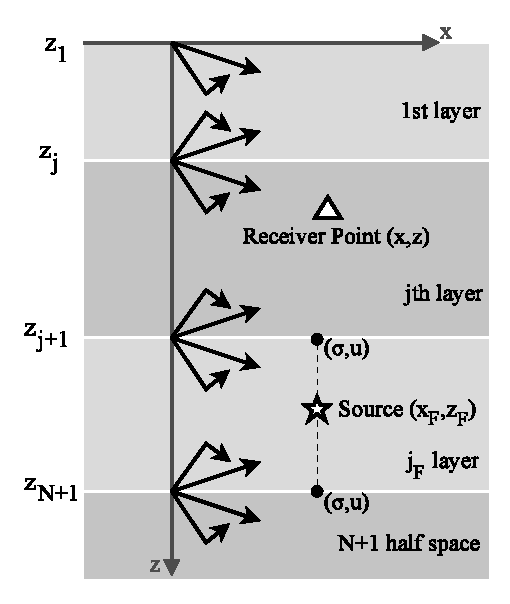
\includegraphics{layeredandsource}
		\caption{Layered half-space showing the plane wave representation of the diffracted field and the source represented as interface traction and displacement discontinuities.}
		\label{figlayeredsoil}
\end{figure}
%In the absence of inclusions $u^{(0)} + u^{(l)}$ 

\section{Discretization}
\section{Testing of the method}
\section{Results}
\section{Discussion}
\section{Conclusions}
\section{Acknowledgments}
\section{References}
% compilar latex, luego BibTex, luego latex dos veces
\bibliographystyle{plain}
\bibliography{./bibliografia}
\section{Appendix A}
\section{Appendix B}
\end{document}

